\section{Tecnologías Utilizadas}

En este capítulo se describen las tecnologías, librerías y servicios utilizados para el desarrollo
del sistema.

La base de datos seleccionada para almacenar las revisiones de los artículos wiki, llamada MongoDB,
y la definición de las características que facilitan el escalamiento horizontal de los datos, tales como: la réplicación,
que permite brindar un servicio con alta disponibilidad; y las particiones, que se refieren a la capacidad
que tiene MongoDB para dividir los datos almacenados en subgrupos entre los múltiples miembros del sistema.

Celery y RabbitMQ, que permiten la creación de una cola de tareas para que puedan ser ejecutadas de forma asíncrona,
disminuyendo los cuellos de botella y así optimizar de cierta manera los tiempos de respuesta y la eficiencia
general del sistema.

Flask, el microframework de Python, el cual permite el desarrollo de aplicaciones web
sin la inclusión componentes innecesarios, y en este caso, permite la creación de un servicio API que aplicaciones
de terceros pueden consumir para la extracción y consulta de las revisiones de los artículos wiki.

Y por último, Docker, que sirve como una herramienta para emular un ambiente distribuido en donde
se van a ejecutar los múltiples nodos tanto de la base de datos, como los servicios de Celery y RabbitMQ, y
las múltiples instancias del servicio API.

\subsection{Mongo}

MongoDB es una base de datos NoSQL (no solo SQL) orientada a documentos. Almacena
datos en una representación binaria llamada BSON (Binary JSON), la cual extiende
las capacidades de un objeto JSON (JavaScript Object Notation) para representar
tipos de datos como enteros, punto flotante, fechas, datos binarios, arreglos y sub-documentos o
documentos embebidos. Cada documento pertenece a un grupo llamado colección, los cuales son el
equivalente a las tablas de una base de datos relacional.

MongoDB posee un conjunto de  características que permiten la escalabilidad de una aplicación, entre ellas,
provee la habilidad e implementar la distribución geográfica de datos (sharding). Esto permite a la
base de datos ser escalada de forma horizontal con el uso de un conjunto de componentes de hardware o mediante
de la nube (cloud).

Adicionalmente, MongoDB \cite{10} está diseñado para ser ejecutado en un sistema de múltiples nodos, por lo tanto,
en la presencia de un escalamiento horizontal, incluye la capacidad para la replicación
y sincronización de datos entre todos los componentes del sistema. De esta manera se garantiza la posibilidad
de implementar un servicio con alta disponibilidad.

\subsubsection{Replicación}

La replicación permite la redundancia de datos y el aumento de disponibilidad de los mismos en aplicaciones distribuidas.
Hace uso de múltiples servidores conectados entre sí y genera una réplica de los datos en cada uno de ellos, de
esta manera se obtiene cierto nivel de tolerancia a fallos en caso de que un servidor de base de datos falle.
También es posible mantener copias adicionales para propósitos específicos como recuperación en casos de desastre,
reportes o respaldos \cite{11}.

En MongoDB se hace uso de grupos de réplica (replica sets) para almacenar las copias de datos en múltiples
servidores de base de datos. Un grupo de replica previene los tiempos de inactividad de la base de datos
en caso de errores y ayuda a escalar las operaciones de lectura. La recuperación de un miembro del grupo de
replica se realiza de forma automática. En un grupo de replica cualquier miembro puede actuar como nodo principal
y el resto como secundario, por lo tanto, en caso de fallas de red o de hardware, un miembro del grupo
puede tomar el puesto de nodo primario después de haber sido elegido siguiendo un conjunto de reglas predefinidas.

Un grupo de réplicas esta conformado por un nodo principal que realizará todas las operaciones de escritura, múltiples nodos
secundarios y un nodo árbitro opcional, tal cual como lo muestra figura \ref{fig:replicas}:

\begin{figure}[H]
	\centering
		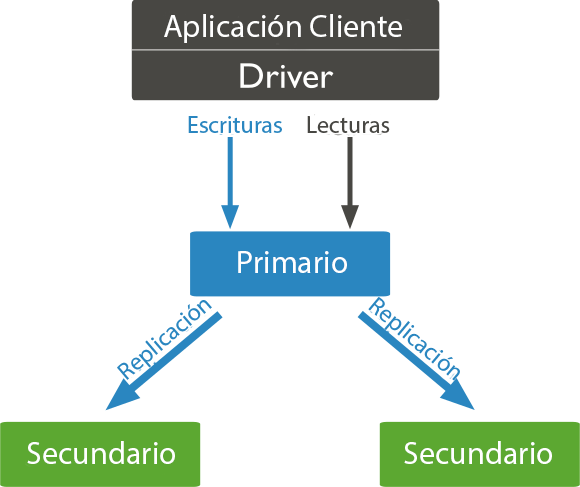
\includegraphics[width=.6\textwidth]{figures/replicas}
	\caption{Componentes de un grupo de replicas en MongoDB y su interacción con una aplicación cliente}
	\label{fig:replicas}
\end{figure}

Para poder crear estos grupos es necesario tener un mínimo de tres nodos y escalar en números impares. Esto se
debe a que cuando los componentes del grupo realicen la votación para elegir el nodo principal, se elimina la posibilidad de un
empate y el ganador es elegido de inmediato.

En la figura \ref{fig:heartbeat} se puede observar como los nodos del grupo se envían mensajes de diagnostico (heartbeats) para determinar si sus vecinos son accesibles o no.
En caso de que uno de estos heartbeat no obtenga una respuesta en 10 segundos, se marca dicho
destinarlo como inaccesibles.

\begin{figure}[H]
	\centering
		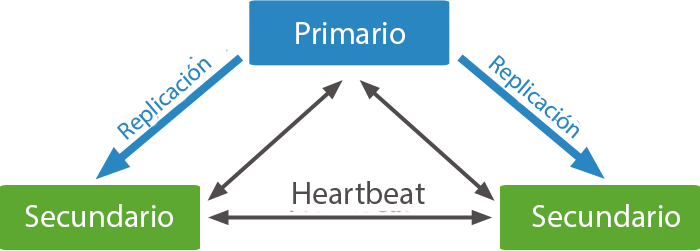
\includegraphics[width=.6\textwidth]{figures/heartbeat}
	\caption{Heartbeats en un grupo de replicación de MongoDB}
	\label{fig:heartbeat}
\end{figure}


Los nodos secundarios se encargan de leer los datos presentes en el nodo primario y crear sus propia replica o copia del mismo.
Si, por alguna razón, el nodo primario deja de estar disponible, un nodo secundario elegible ejecutará una votación para elegir el siguiente nodo primario, tal como lo muestra la figura \ref{fig:failover}.
El primer nodo secundario en llevar a cabo la elección y recibir la mayoría de los votos se convierte en el nuevo nodo primario.

\begin{figure}[H]
	\centering
		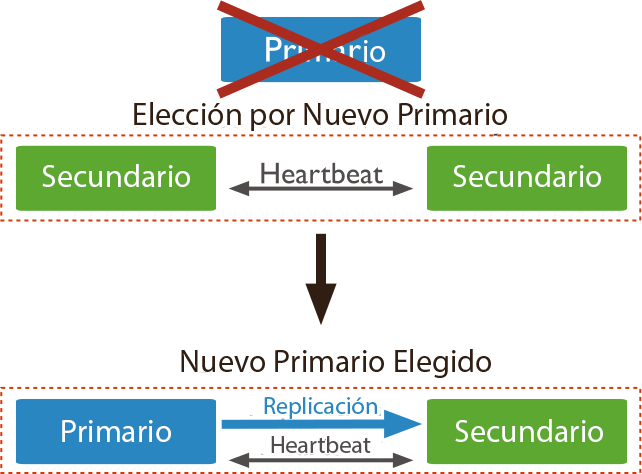
\includegraphics[width=.6\textwidth]{figures/failover}
	\caption{Proceso de elección de nuevo nodo primario}
	\label{fig:failover}
\end{figure}

\subsubsection{Particiones}

El proceso de partición (sharding) es un método de escalamiento horizontal que distribuye datos entre múltiples máquinas.
Cada conjunto de datos alojado en una máquina es llamado partición (shards), y su acceso es completamente transparente para las aplicaciones.
Este método permite atacar las limitaciones de hardware provenientes del uso de un solo servidor, tales como los cuellos de botella o capacidad de almacenamiento \cite{13}.

En MongoDB, un grupo de partición (sharded cluster) consiste de tres componentes:

\begin{itemize}
\item Partición: Cada partición contiene un subconjunto de los datos y pueden ser implementados como un grupo de réplica.

\item mongos: mongos es un servicio que actuá como interfaz entre las aplicaciones cliente y el grupo de partición, también es llamado
query router.

\item Servidores de Configuración: Los servidores de configuración almacenan meta datos y los atributos de configuración del cluster, y
al igual que las particiones, también pueden ser implementados como un grupo de réplica.
\end{itemize}

En la figura \ref{fig:sharding} se puede apreciar los componentes del cluster de particiones y la interacción entre los mismos:

\begin{figure}[H]
	\centering
		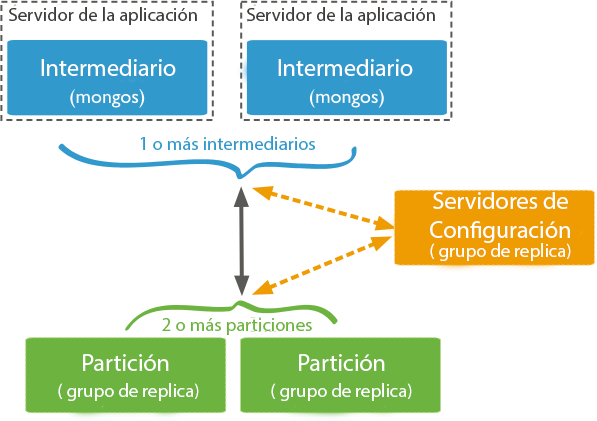
\includegraphics[width=.7\textwidth]{figures/sharding}
	\caption{Componentes de un cluster de particiones}
	\label{fig:sharding}
\end{figure}

Para distribuir los documentos de un colección es necesario el uso de una llave de partición (shard key). Un shard key es uno o
múltiples campos inmutables que comparten todos los documentos de una colección. Una colección particionada solo puede tener un shard key
y la misma no puede ser cambiada después de haberse ejecutado el proceso de sharding.

MongoDB genera particiones de datos a nivel de colección, distribuyendo los documentos de una colección entre los miembros
del cluster de particiones. Una base de datos puede tener una combinación de colecciones particionadas y no particionadas.
Las colecciones particionadas son distribuidas entre cada partición del cluster, mientras que las colecciones no particionadas son
almacenadas en una partición especial llamada primaria.

El acceso a una base de datos particionada en MongoDB es completamente transparente para cualquier aplicación de cliente, tan
solo es necesario saber la dirección IP o nombre del equipo (hostname) y el puerto en el cual se ejecutará el query router.
La figura \ref{fig:sharding_apps} detalla la interacción entre una aplicación de cliente con una base de datos MongoDB con particiones:

\begin{figure}[H]
	\centering
		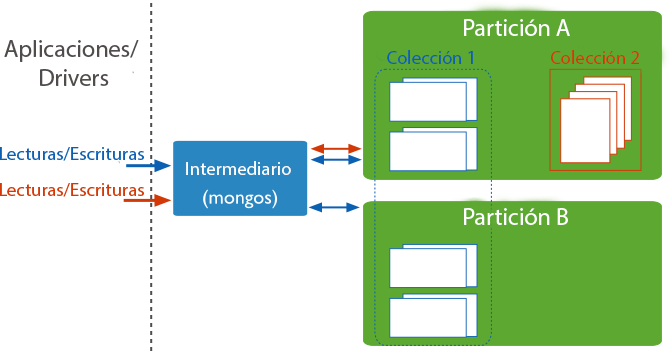
\includegraphics[width=.7\textwidth]{figures/sharding_apps}
	\caption{Interacción entre una aplicación cliente y una base de datos MongoDB particionada}
	\label{fig:sharding_apps}
\end{figure}

MongoDB ofrece múltiples estrategias o políticas de particionamiento que permiten a un administrador de base de datos
o desarrollador distribuir los datos entre los miembros del cluster.

\begin{itemize}

\item Range Sharding. Los documentos son divididos en rangos contiguos determinados por el valor del shard key. Se toma el valor
mínimo y máximo de todos las particiones y se generan N grupos, ordenados de menor a mayor por el shard key y separados por rangos,
tal cual se puede observar en la figura \ref{fig:ranged_sharding}:

\begin{figure}[H]
	\centering
		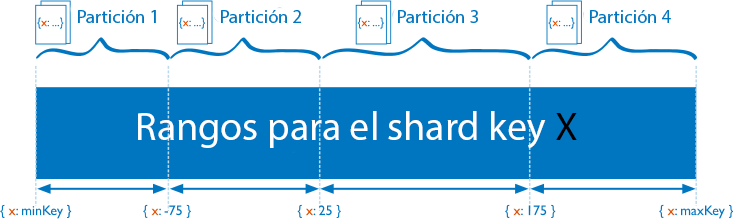
\includegraphics[width=.7\textwidth]{figures/ranged_sharding}
	\caption{Range Sharding de datos en MongoDB}
	\label{fig:ranged_sharding}
\end{figure}

\item Hash Sharding. Los documentos son distribuidos acorde al valor del hash MD5 del shard key. Una vez calculado el valor del hash, se
dividen los datos en subgrupos separados en rangos. Este método garantiza la distribución uniforme de los documentos entre las particiones.
MongoDB es quien calcula el valor del hash, por lo que las aplicaciones que interactúen con la base de datos no necesitan llevar a cabo este paso.
Un ejemplo de esto se puede apreciar en la figura \ref{fig:hashed_sharding}:

\begin{figure}[H]
	\centering
		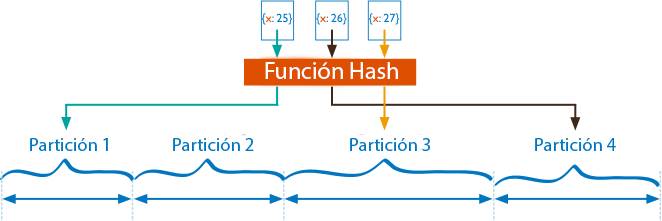
\includegraphics[width=.7\textwidth]{figures/hashed_sharding}
	\caption{Hashed Sharding de datos en MongoDB}
	\label{fig:hashed_sharding}
\end{figure}

\item Zone Sharding. Provee las herramientas para la definición de las reglas que definen el lugar en que serán almacenados los datos
en el cluster. Se crean zonas de datos particionados basados en el shard key, y es posible asociar cada zona con uno o más particiones
del cluster. Zone Sharding permite establecer políticas en donde se puede almacenar y localizar datos por región geográfica, por
servicios específicos de una aplicación, e incluso por la configuración de hardware en caso de tener una arquitectura de almacenamiento
por capas.

\begin{figure}[H]
	\centering
		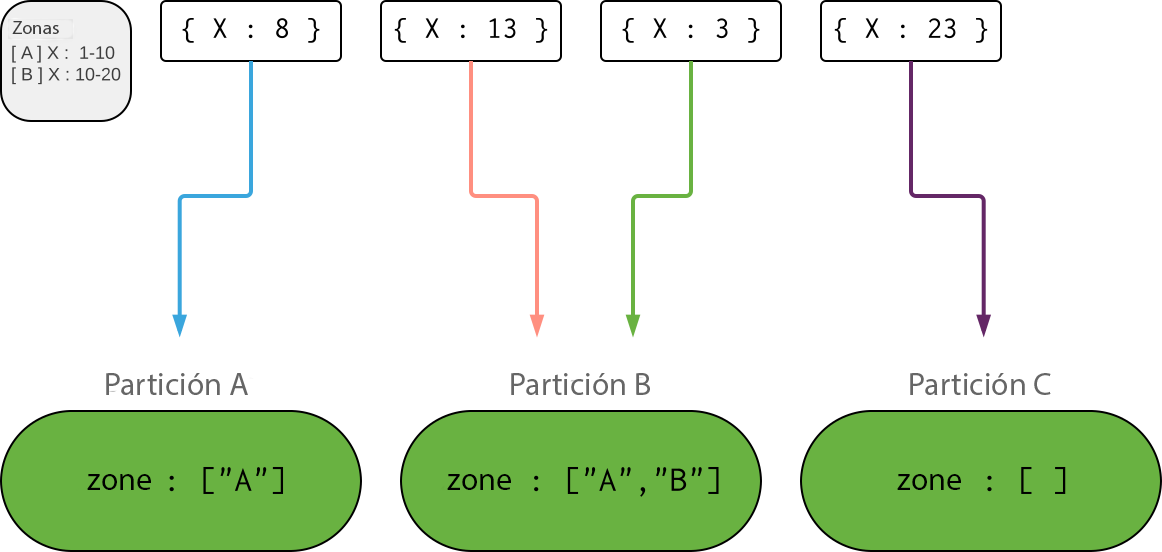
\includegraphics[width=.9\textwidth]{figures/zone_sharding}
	\caption{Zone Sharding de datos en MongoDB}
	\label{fig:zone_sharding}
\end{figure}

\end{itemize}

\subsubsection{PyMongo}

PyMongo es una librería  de Python que permite la interacción con una base de datos MongoDB.
Básicamente se encarga de mantener un canal de comunicación con la base de datos
y ejecutar consultas \cite{17}.

PyMongo posee la cualidad de funcionar correctamente si es ejecutado
simultáneamente por múltiples hilos, esta característica es llamada: segura en hilos
(thread-safe) \cite{18}.
PyMongo, tiene incorporado una agrupación de conexiones abiertas a
la base de datos para que los hilos de una aplicación puedan reutilizar dichas
conexiones al momento de ejecutar múltiples consultas o actualizaciones. Esta
característica ayuda a incrementar el rendimiento puesto que PyMongo no establece
una nueva conexión con la base de datos por cada que necesite ejecutar, de esta forma
se evita la sobrecarga que la apertura de conexión pueda causar.

\subsection{Celery}

Celery es una herramienta que permite creación de colas y tareas asíncronas basada en la transmisión de mensajes distribuidos.
Esta concentrado en la ejecución de operaciones en tiempo real, y a su vez, también soporta la planificación de tareas.

Las colas de tareas son usadas como un mecanismo para la distribución de trabajo entre múltiples hilos o máquinas.
Las entradas de estas colas son ejecutadas de forma concurrente en uno o más componentes llamados workers, quien constantemente verifican si existe una tarea en la cola para ser ejecutada.
Estas tareas pueden ser ejecutadas en segundo plano o de forma sincrónica, es decir, que esperan a que la tarea anterior culmine.

Celery realiza la transmisión de mensajes haciendo uso de un agente intermediario llamado broker.
Para iniciar una tarea un cliente agrega un mensaje a la cola, el broker toma este mensaje y se lo envía a algún worker disponible, por último, una vez el worker recibe el mensaje ejecuta la tarea.
Este proceso se puede observar en la figura \ref{fig:celery}:

\begin{figure}[H]
	\centering
		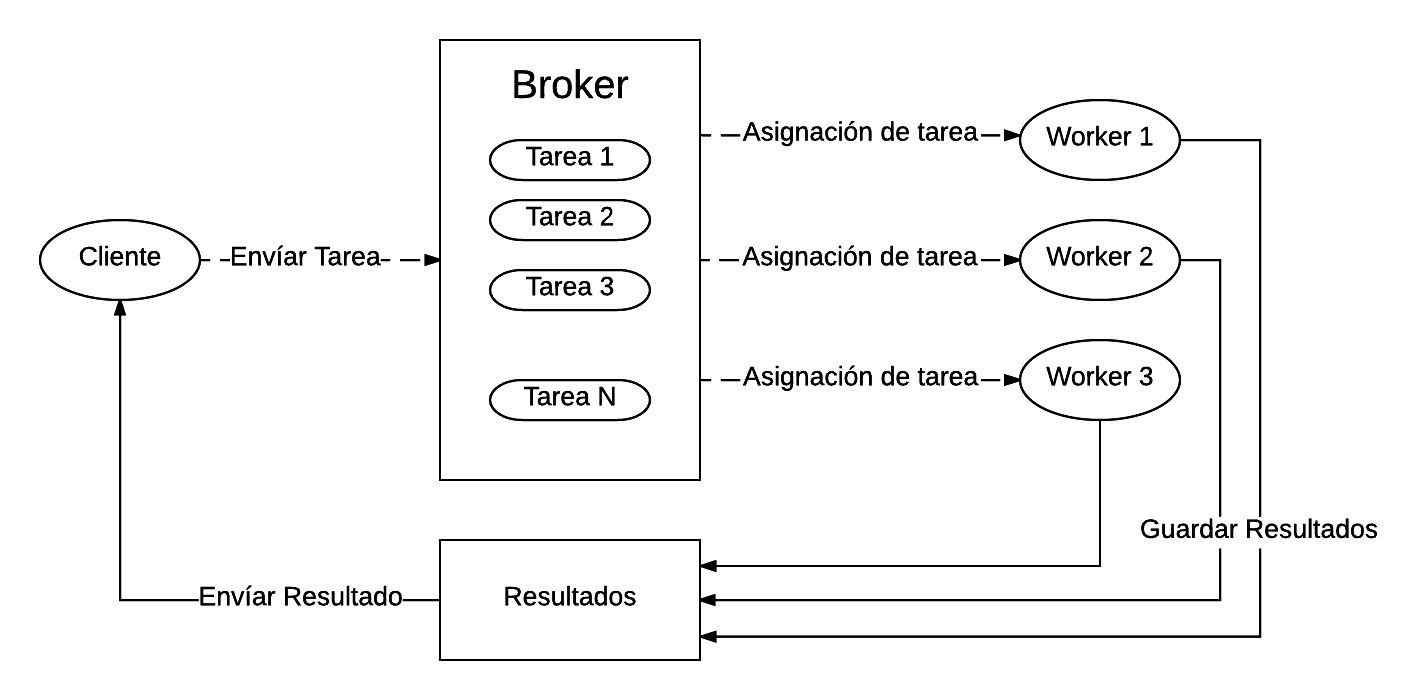
\includegraphics[width=.9\textwidth]{figures/celery}
	\caption{Flujo de trabajo en la asignación de tareas de Celery}
	\label{fig:celery}
\end{figure}

\subsection{RabbitMQ}

RabbitMQ es un intermediario para la transmisión de mensajes que sirve como plataforma para que los mensajes enviados
en una aplicación sean almacenados de forma temporal durante el proceso de comunicación \cite{14}.

El uso de la mensajería en una aplicación permite la conexión entre múltiples componentes de la misma, ya sea para enviar notificaciones, datos, tareas asíncronas o suscripción a un servicio.
Un mensaje puede incluir cualquier tipo de información, por ejemplo, puede contener datos relacionados con un proceso o tarea, una notificación, e incluso el resultado de una operación.
RabbitMQ almacena estos mensajes y los coloca en una cola hasta que alguna aplicación se conecta a él y toma dicho mensaje de la cola.

RabbitMQ hace uso del protocolo AMPQP (Advanced Message Queuing Protocol), el cual esta diseñado para la transmisión
de mensajes de aplicación entre sistemas usando, entre otras, una combinación de técnicas como: almacenamiento y reenvío, en donde
los datos son almacenados en un componente intermediario de forma temporal y después enviados al destinatario final u a otro
intermediario \cite{15}; y el patrón publicación-suscripción, en donde el emisor del mensaje no envía datos a un destinatario
en específico, sino que existe un miembro llamado suscriptor quien decide o no si recibir los mensajes publicados por el emisor \cite{16}.

En la figura \ref{fig:workflow_rabbitmq} se puede apreciar un flujo de trabajo simple en la emisión y suscripción de mensajes usando RabbitMQ:

\begin{figure}[H]
	\centering
		
\includegraphics[width=1\textwidth]{figures/workflow_rabbitmq}
	\caption{Flujo de trabajo de la emisión y suscripción de mensajes en RabbitMQ}
	\label{fig:workflow_rabbitmq}
\end{figure}

\subsection{Flask}

Flask es un framework (microframework) para el desarrollo aplicaciones
web. Esta característica se refiere a que tiene como objetivo mantener
el núcleo de la aplicación de simple pero extensible \cite{19}.
Es decir, no tiene limitaciones ni ofrece herramientas en el uso de servidores de
bases de dato a usar, motores de plantillas, manejadores de correos o validaciones de
formulario.
En cambio, es capaz de soportar extensiones y librerías que agregan
estas funcionalidades a la aplicación de tal forma que parecieran ser implementadas por Flask.

El objetivo de Flask es permitir la construcción de una base sólida para todas las
aplicaciones, y que cualquier otro requerimiento o módulo necesario, que sea
implementado por el desarrollador o por la inclusión de extensiones \cite{20}.

\subsection{Nginx}

Nginx es un servidor HTTP que también funciona como: un proxy reverso, servidor
proxy IMAP/POP3 e inclusive como software para el manejo de balance de carga [16].
Puede ser usado para servir contenido HTTP estático y dinámico en la red haciendo uso
de FASTCGI, manejadores SCGI para scripts, servidores de aplicación WSGI o módulos
de Phusion Passenger.

Nginx no utiliza múltiples hilos para manejar solicitudes, en cambio, hace uso de un
solo hilo y la implementación del paradigma de la programación dirigida por eventos,
en donde el manejo de las peticiones recibidas por este servidor van determinados por
los sucesos que ocurran en el sistema.
La arquitectura modular dirigida por eventos de
Nginx permite proveer un rendimiento predecible en ambientes de alta carga de
trabajo.

La capacidad de Nginx de ser utilizado como proxy reverso tiene diversos usos.
El uso de un proxy es típicamente usando para distribuir la carga de peticiones
entre múltiples servidores, mostrar contenido de múltiples servicios web de forma transparente,
e incluso transferir peticiones a un servidor por protocoles diferentes a HTTP \cite{22}.

Un ejemplo de como seria el flujo de trabajo para atender una petición con un proxy reverso se puede apreciar en la figura \ref{fig:nginx_reverse_proxy}:

\begin{figure}[H]
	\centering
		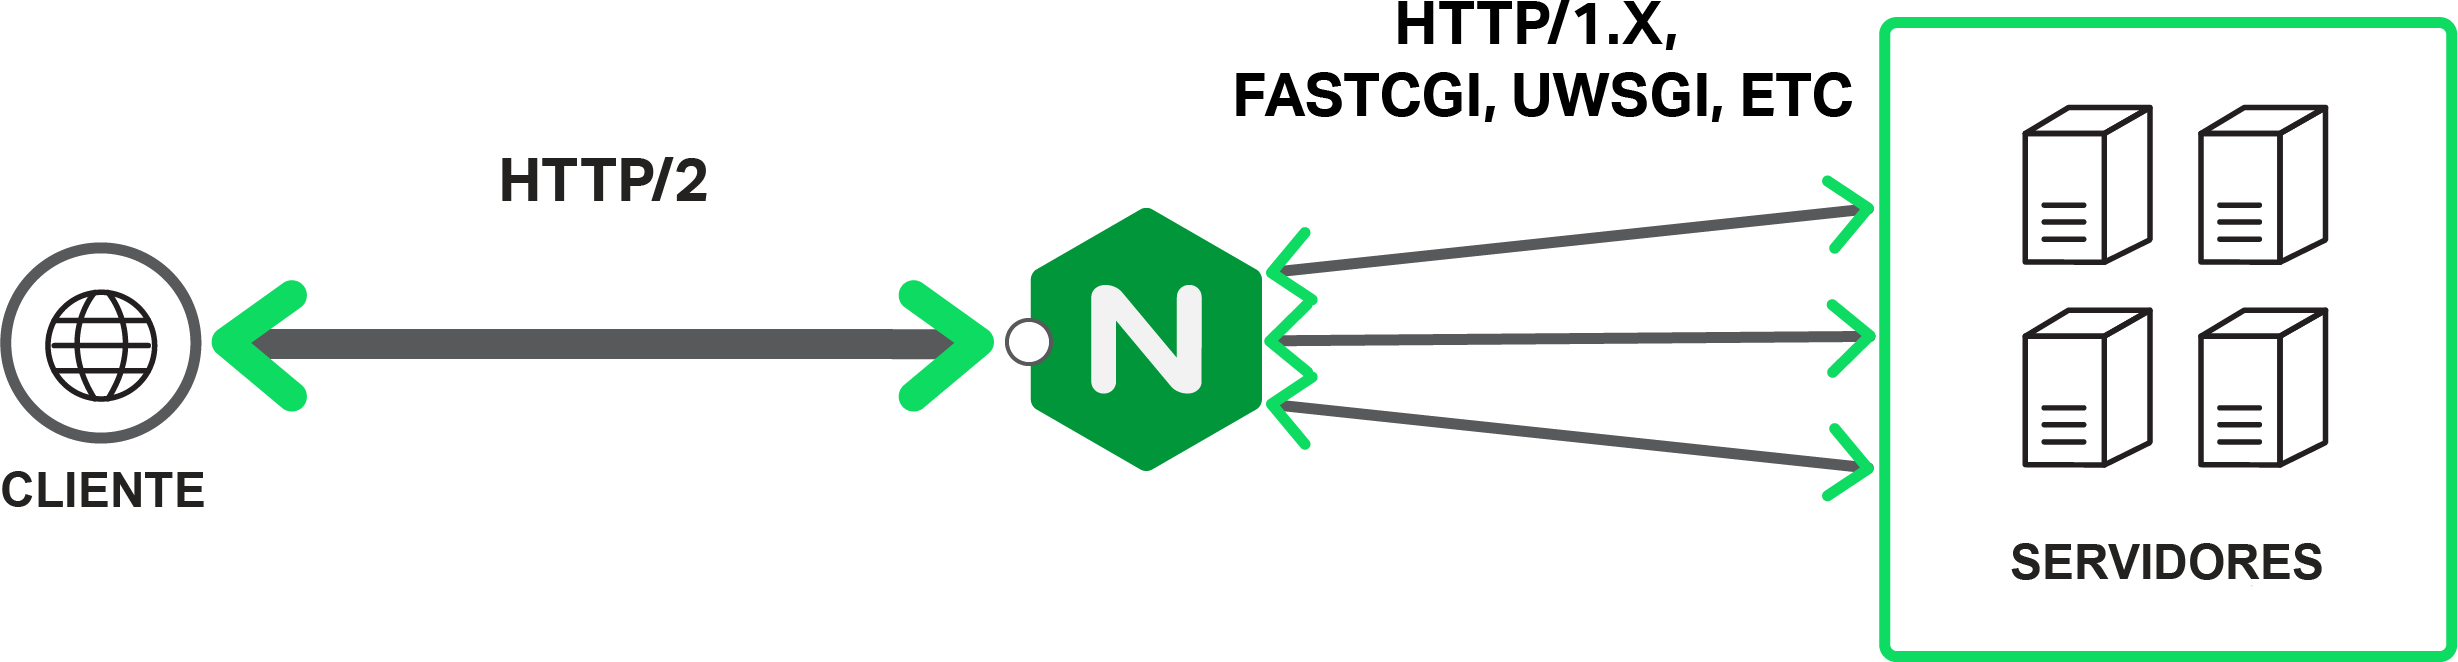
\includegraphics[width=.9\textwidth]{figures/nginx_reverse_proxy}
	\caption{Atención de peticiones con el uso de proxy reverso de Nginx}
	\label{fig:nginx_reverse_proxy}
\end{figure}

Dado una aplicación cliente que emite una petición al servicio, es Nginx es quien recibe la petición y procede a elegir cual servidor
atenderá la petición. Cada servidor ejecuta la aplicación haciendo uso de tecnologías como UWSGI, FASTCGI, SCGI, etc. Una vez que el
servidor atiende la petición, envía la respuesta devuelta a Nginx y este último la reenvía al cliente.


\subsection{Docker}

Docker es una plataforma para la automatización en el despliegue de aplicaciones dentro de paquetes llamados contenedores de software,
los cuales contienen todos los elementos que permiten su ejecución en cualquier sistema operativo.

Un contenedor de software es una manera de empaquetar software en un formato en el cual puede ser ejecutado de forma aislada en un sistema
operativo. Solo se empaqueta el código, sus librerías, dependencias y configuraciones necesarias para que el
software funcione de forma adecuada sin ejecutar un sistema operativo por completo.
De esta manera se generan sistemas independientes, eficientes y ligeros que garantizan
que el software siempre se ejecutará de la misma manera sin importar el ambiente \cite{21}.

Los contenedores de software están conformados por dos componentes: una imagen y un contenedor.

\begin{itemize}
\item Imagen: es un paquete ejecutable aislado que incluye todo lo necesario para ejecutar un software, incluyendo código,
librerías, variables de entorno y archivos de configuración.

\item Contenedor: es una instancia de una imagen. Su ejecución, por defecto, esta aislada del ambiente de la máquina anfitrión,
de tal forma que solo accede a los archivos y/o puertos del anfitrión si fue configurado para ello.
\end{itemize}

Los contenedores ejecutan aplicaciones directamente en el kernel de la máquina anfitrión, por lo que tienen mejor rendimiento que una máquina virtual que solo tiene acceso virtual a los recursos del anfitrión.

La figura \ref{fig:docker_vm} muestra cómo las máquinas virtuales ejecutan sistemas operativos completos sobre la máquina anfitrión:

\begin{figure}[H]
	\centering
		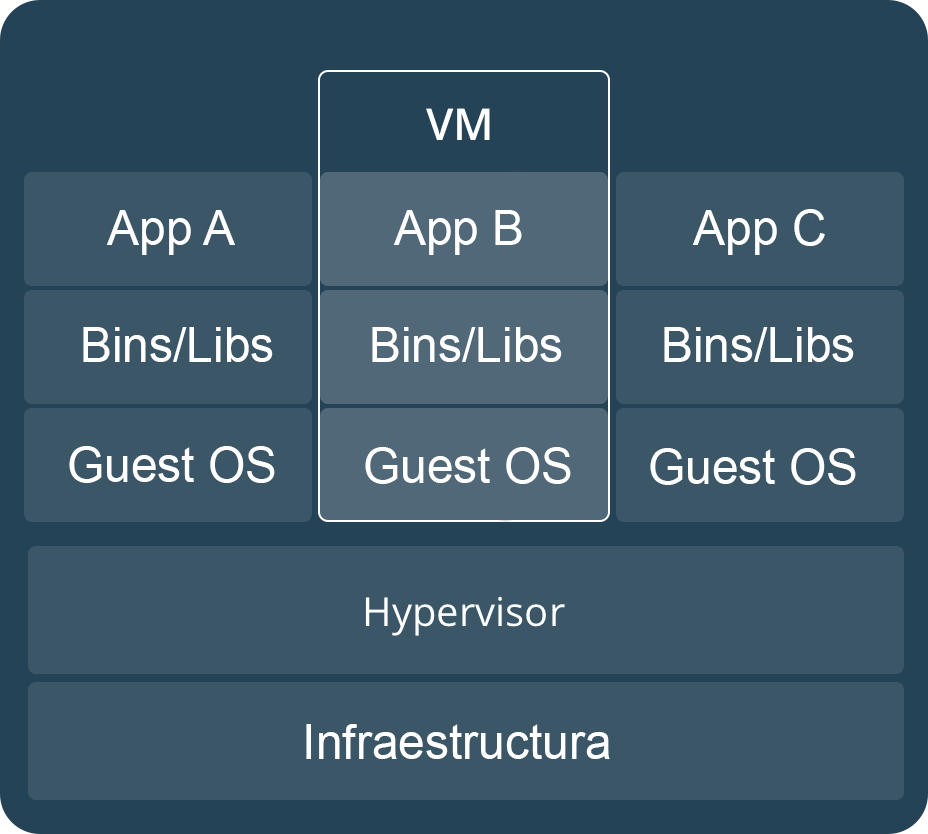
\includegraphics[width=.9\textwidth]{figures/docker_vm}
	\caption{Diagrama de componentes de una Maquina Virtual}
	\label{fig:docker_vm}
\end{figure}

En cambio, los contenedores pueden compartir un mismo kernel, la única información que necesita tener la imagen del contenedor es el ejecutable y sus dependencias.
En la figura \ref{fig:docker_container} se puede apreciar como cada contenedor se ejecutará como una aplicación aislada sobre el sistema operativo:

\begin{figure}[H]
	\centering
		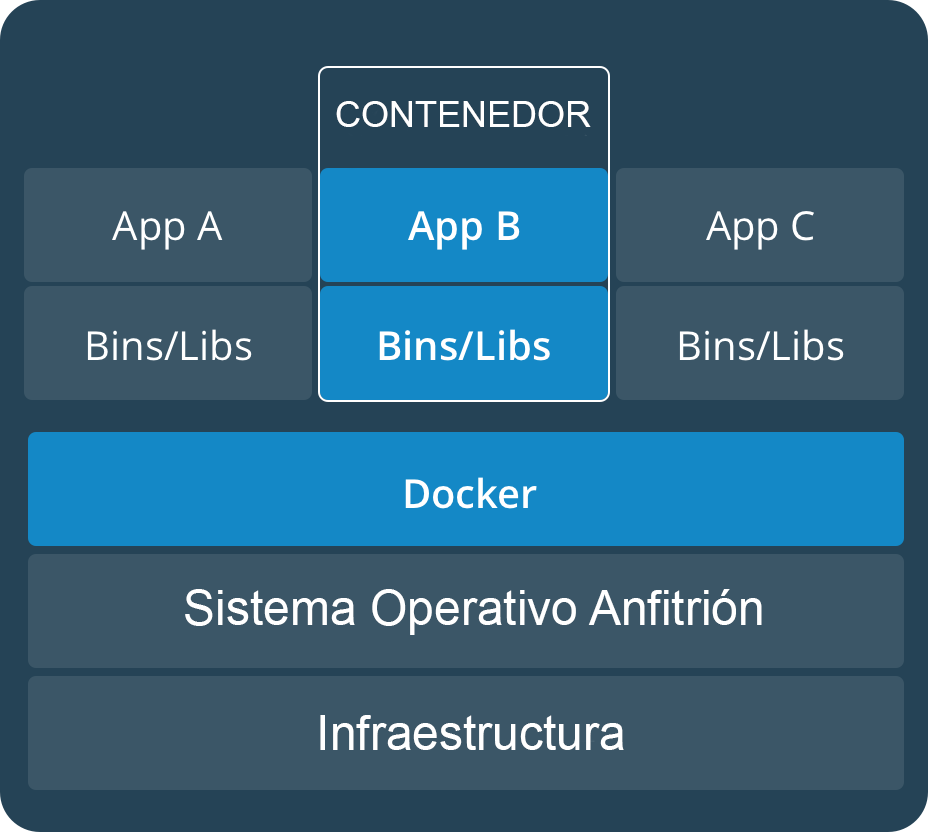
\includegraphics[width=.8\textwidth]{figures/docker_container}
	\caption{Diagrama de componentes de un Contenedor}
	\label{fig:docker_container}
\end{figure}

Docker permite la creación de redes y espacios de almacenamiento, llamados volúmenes, que pueden ser asignados a uno o múltiples contenedores a la vez.
De esta forma, es posible conectar varios contenedores entre sí mediante una red y compartir archivos.
Esto permite gestionar múltiples contenedores para que se ejecuten como un sistema distribuido,
en donde es posible, y si los recursos lo permiten, desplegar nuevos nodos que cumplan las funciones como:
un miembro en una réplica de base de datos, un worker de celery e incluso un servicio como RabbitMQ.
